Das Logik-Rätsel Dedalo wird auf einem $n\times n$-Feld gespielt.
Darauf sind die Zahlen $1,\dots,k$ jeweils genau zweimal eingetragen,
ein Feld kann aber höchstens eine Zahl enthalten.
Gleiche Zahlen sollen jetzt durch einen Weg verbunden werden, wobei jedes Feld
genau einmal von genau einem Weg getroffen werden darf,
Wege können sich also nicht kreuzen.
Es ist muss jedes Feld von einem Weg besucht sein, es ist nicht zulässig,
dass ein Feld leer bleibt.

Hier ist ein Dedalo-Rätsel mit eingezeichneter Lösung:
\begin{center}
\def\d{0.6}
\def\knoten#1#2#3{\node at ({#1*\d},{#2*\d}) {#3};}
\def\feld{
	\foreach \t in{0.5,1.5,...,8.5}{
		\draw[line width=0.5pt] ({\t*\d},{-0.5*\d})--({\t*\d},{9.5*\d});
		\draw[line width=0.5pt] ({-0.5*\d},{\t*\d})--({9.5*\d},{\t*\d});
	}

	\draw ({-0.5*\d},{-0.5*\d}) -- ({9.5*\d},{-0.5*\d});
	\draw ({-0.5*\d},{9.5*\d}) -- ({9.5*\d},{9.5*\d});

	\draw ({-0.5*\d},{-0.5*\d}) -- ({-0.5*\d},{9.5*\d});
	\draw ({9.5*\d},{-0.5*\d}) -- ({9.5*\d},{9.5*\d});

	\knoten{6}{2}{1}
	\knoten{9}{9}{1}

	\knoten{0}{0}{2}
	\knoten{8}{9}{2}

	\knoten{3}{3}{3}
	\knoten{3}{9}{3}

	\knoten{6}{1}{4}
	\knoten{9}{1}{4}

	\knoten{1}{0}{5}
	\knoten{9}{0}{5}

	\knoten{7}{4}{6}
	\knoten{7}{9}{6}

	\knoten{4}{5}{7}
	\knoten{6}{4}{7}

	\knoten{1}{8}{8}
	\knoten{5}{8}{8}

	\knoten{1}{9}{9}
	\knoten{2}{3}{9}

	\knoten{0}{2}{10}
	\knoten{0}{9}{10}
}
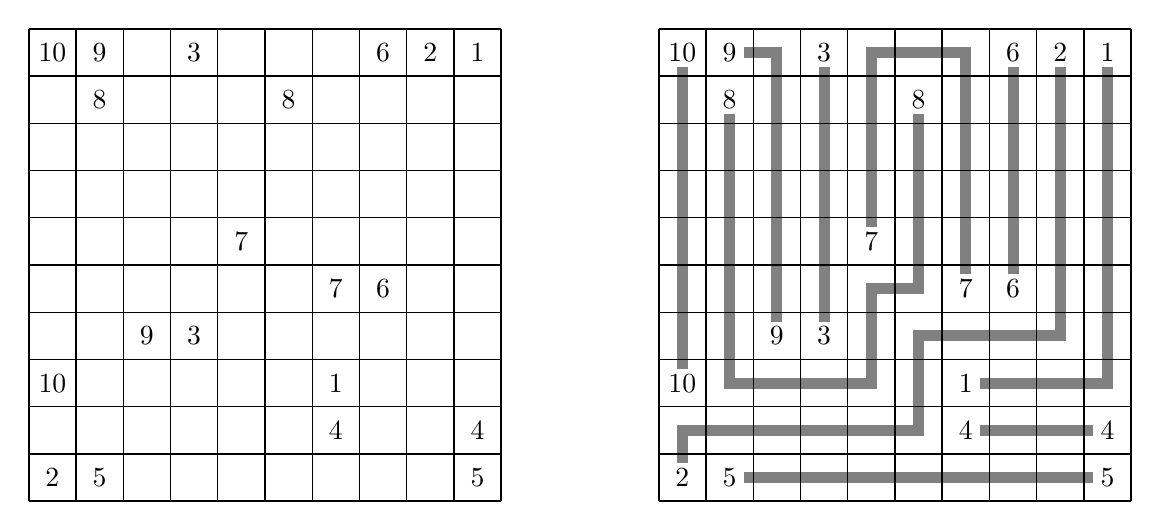
\begin{tikzpicture}[>=latex,thick]

\begin{scope}[xshift=-4cm]
\feld
\end{scope}

\begin{scope}[xshift=4cm]
\draw[line width=4pt,color=gray]
({6.3*\d},{2*\d})--
({9*\d},{2*\d})--
({9*\d},{8.7*\d});
\draw[line width=4pt,color=gray]
({0*\d},{0.3*\d})--
({0*\d},{1*\d})--
({5*\d},{1*\d})--
({5*\d},{3*\d})--
({8*\d},{3*\d})--
({8*\d},{8.7*\d});
\draw[line width=4pt,color=gray]
({3*\d},{3.3*\d})--
({3*\d},{8.7*\d});
\draw[line width=4pt,color=gray]
({6.3*\d},{1*\d})--
({8.7*\d},{1*\d});
\draw[line width=4pt,color=gray]
({1.3*\d},{0*\d})--
({8.7*\d},{0*\d});
\draw[line width=4pt,color=gray]
({7*\d},{4.3*\d})--
({7*\d},{8.7*\d});
\draw[line width=4pt,color=gray]
({4*\d},{5.3*\d})--
({4*\d},{9*\d})--
({6*\d},{9*\d})--
({6*\d},{4.3*\d});
\draw[line width=4pt,color=gray]
({1*\d},{7.7*\d})--
({1*\d},{2*\d})--
({4*\d},{2*\d})--
({4*\d},{4*\d})--
({5*\d},{4*\d})--
({5*\d},{7.7*\d});
\draw[line width=4pt,color=gray]
({2*\d},{3.3*\d})--
({2*\d},{9*\d})--
({1.3*\d},{9*\d});
\draw[line width=4pt,color=gray]
({0*\d},{2.3*\d})--
({0*\d},{8.7*\d});


\feld
\end{scope}


\end{tikzpicture}
\end{center}
Zeigen Sie, dass eine nichtdeterministische Turing-Maschine in polynomieller
Zeit entscheiden kann, ob ein Dedalo-Rätsel lösbar ist.

\thema{NP}
\thema{polynomieller Verifizierer}

\begin{loesung}
Die Frage ist sicher entscheidbar, indem man alle möglichen Wege
durchprobiert und prüft, ob sie die verlangten Bedingungen erfüllen.

Um die gestellte Frage zu beantworten, müssen wir einen polynomiellen
Verifzierer konstruieren.
Als Lösungszertifikat verlangen wir die Wege. 
Der Verifikationsalgorithmus muss folgendes überprüfen:
\begin{center}
\begin{tabular}{c|p{8cm}|c}
Schritt&Algorithmus&Laufzeit
\\
\hline
1&Für jedes Feld kontrollieren, dass höchstens ein Weg dort durchgeht& $O(n^2)$
\\
2&Für jeden Weg kontrollieren, dass die Felder an den Enden die
gleiche Nummer haben& $O(n^4)$
\\
3&Für jedes Feld kontrollieren, dass ein Weg dort durchgeht& $O(n^2)$
\\
\hline
&Total&$O(n^4)$
\end{tabular}
\end{center}
Dieser Verifizierer hat offensichtlich polynomielle Laufzeit $O(n^4)$ und
daher kann eine nichtdeterministische Turing-Maschine in polynomieller Zeit
entscheiden, ob ein Dedalo-Rätsel lösbar ist.
\end{loesung}

\begin{bewertung}
Entscheidbarkeit ({\bf E}) 1 Punkt,
Verifizierer ({\bf V}) 1 Punkt,
Zertifikat ({\bf Z}) 1 Punkt,
Algorithmus ({\bf A}) 1 Punkt,
Laufzeitschätzung ({\bf L}) 1 Punkt,
Schlussfolgerung ({\bf S}) 1 Punkt.
\end{bewertung}




